\documentclass{ctuthesis}

%\usepackage[disable]{todonotes} % don't generate todos to pdf
\usepackage{todonotes} % show todos in generated pdf

\usepackage{indentfirst}

\ctusetup{
    xfaculty = F3,
    mainlanguage = english,
    titlelanguage = english,
    title-english = {Unassisted project report},
    title-czech = {Zpráva Samostatného projektu},
    department-english = {Department of Computer Science},
    author = {Lukáš Forst},
    supervisor = {Ondřej Vaněk, Ph.D.},
    month = 1,
    year = 2019,
}

\ctuprocess


\begin{document}
    \maketitle

    \chapter{Introduction}\label{ch:introduction}
The globalization of the world’s economies is a major challenge to local industry 
and it is pushing the manufacturing sector to the transformation called \textit{Industry 4.0} \cite{industry40}.
In order to become more competitive, 
manufacturers need to embrace emerging technologies, 
such as advanced analytics, artificial intelligence 
and mathematical optimization to improve their efficiency and productivity.

Specifically manufacturing industry sector,
which have high production costs,
faces multiple problems,
where employing mathematical optimization can reduce cost or improve efficiency of the process.
Taking as en example the car manufacturers,
there are many processes,
that can be optimized to reduce their cost or to use needed resources more efficiently,
such as an internal logistics, car parts transportation, parts stocking, cars manufacturing 
and the allocation of the various types of resources.
These optimization challenges are often solved by the proprietary software systems with included optimization engine,
where the one problem domain is usually handled by the single program operating specifically with such domain.

These applications typically have an user interface for the data visualization
and an engine running an optimization algorithm.
Although the data visualization part of the application does not require powerful hardware,
the immense complexity of the mathematical optimization problems 
and thus the performance requirements for such optimization engine solving them, are not always satisfiable.
Moreover,
the computer performance is finite resource
and it cost money paid for the computer components or for the electricity used.
For that reasons,
the optimization software systems have often limited access to the computer resources.
In addition,
this computer performance is not used all the time,
since the typical usage of such application lays mainly in data visualization,
hence the performance, required only when the optimization engine is running, is unused.

Using such software architecture seems to be highly inefficient,
since the instances, that are in time $t$ running the optimization algorithm, are overwhelmed 
and in the same time $t$,
the applications, that are not running the optimization tasks,
do not use their powerful computer resources at all.

The potential solution for this problems lays in microservices architecture,
where the parts of the applications are independent and able to run separately.
Using this approach enables distributed computing
and therefore outsourcing the demanding optimization engine to more powerful servers.
This approach solves the lack of resources for the optimization engine on the less powerful servers,
but it also introduce new challenge in the load balancing of the servers,
where the optimization engine is being executed.

In this thesis we would like to present the load balancer specifically developed for the optimization algorithms,
which should minimize resources wasting 
and increase the performance using correct utilization distribution across the multiple instances of such algorithms.

\section{Thesis goals}\label{sec:thesis-goals}

This thesis extensively studies and describes state of the art algorithms used for computational task scheduling
and load balancing in section \ref{sec:load-balancing}. 
It also brings overview of various optimization problems, techniques and algorithms 
that are being used in real-life situations to solve diverse industries problems 
in section \ref{sec:optimization-algorithms}.
The complex problem of computational task scheduling is formalized in chapter \ref{ch:problem-formalization}.

Although the main goal is to develop fully functional scheduling system,
mainly because of estimated complexity,
this thesis focuses only on system's core - 
scheduling and load balancing for optimization algorithms in heterogenous distributed environment.

Solution design including final algorithm is proposed in chapter \ref{ch:solution-design}.
In the following chapter (\ref{ch:implementation}),
thesis describes resulting implementation of the load balancing system
and also gives overview of its architecture in the section \ref{sec:architecture}.
Scheduler is then evaluated using multiple simulations in section \ref{sec:simulations}.

To achieve ultimate goal, having fully functional scheduling and load balancing system,
future necessary steps are outlined in section \ref{sec:future-work}.


%    %%
%% Author: lukas
%% 03.01.2019
%%

\chapter{Technical Background}\label{ch:technical-background}

%%
%% Author: lukas
%% 03.01.2019
%%

\section{Optimization Algorithms}\label{sec:optimization-algorithms}

This work does not contain any own algorithm implementation for generic optimization problems,\todo{This is really shity introduction}
instead I would like to use pre-prepared and already implemented optimization solver.
We have many options how to solve optimization problems, I would like to present two of them
- linear optimization and heuristics algorithms.

\subsection{Linear Optimization}\label{subsec:linear-optimization}
Linear optimization (or linear programming) is a method to achieve the best outcome in a mathematical model\todo{I must add more about it since it is important topic}
whose requirements are represented by linear relationships.
The algorithms are widely utilized in company management, such as planning, production, transportation, technology and other issues.

The main benefit of linear optimization is that it provides the best possible solution,
because optimization algorithms are guaranteed to provide optimal solution.
Although almost everything can be represented as linear problem,
linear programming solvers could be unable to provide solution since, in the most cases, computation time grows exponentially.
Even though there are solvers that are able to provide $\epsilon$ (partial) solution,\todo{this need some reference}
this solution can be (and in most cases is) unusable, because is is not optimal at all.

\medskip
\noindent There are plenty of linear programming solvers available.
I would like to highlight following two optimization kits.

\subsubsection{GLPK}\label{subsubsec:glpk}
\textbf{GNU} - \textit{GNU Linear Programming Kit} is a software package intended for solving large-scale linear programming (LP),
mixed integer programming (MIP), and other related problems.
It is a set of routines written in ANSI $C$ and organized in the form of a callable library\cite{web:gnuGlpk}.
Although originally is GLPK written in $C$ programming language,
there is an independent project,
which provides Java-based interface for execution of GLPK via Java Native Interface.
\footnote{Java Native Interface - Interface provided by Java platform to run and integrate non-Java language libraries}

\subsubsection{Google OR-Tools}
\textbf{Google OR-Tools} - OR-Tools is an open source software suite for optimization,
tuned for tackling the world's toughest problems in vehicle routing, flows,
integer and linear programming, and constraint programming\cite{web:googleOrTools}.
Tools contain \textit{Glop} which is Google's custom linear solver.
One of the greatest advantages of Google OR-Tools is great API supporting multiple programming languages - \textit{C++, Python, C\#} and \textit{Java}.


\subsection{Heuristic algorithms}\label{subsec:heuristic-algorithms}
Heuristics algorithms (or HA) are designed to solve optimization problems faster\todo{Same as above, I must add more information about them}
and more efficient fashion than Linear Optimization methods by using different kinds of heuristics and metaheuristics.
In exchange for that, algorithms sacrifice optimality, accuracy, precision, and completeness.
Thus solution provided by HA is not guaranteed to be optimal.
HA are often used to solve various types of NP-complete problems such as
Vehicle Routing, Task Assignment, Job Scheduling or Traveling Salesmen Problem.
Heuristic algorithms are most often employed when approximate solutions are sufficient
and exact solutions are necessarily computationally expensive\cite{papanikolaou2018holistic}.

The main advantage of heuristic algorithms is that they provide quick feasible solution.
Because the implementation of HA is easier than LP and they provide at least feasible solution for optimization problems,
they are solving, they are widely used in organizations that face such optimization problems.
The main downside of HA is the fact, that they can't guarantee that the found solution is the optimal one.

\medskip
\noindent I would like to mention two implementations of heuristics algorithms - OptaPlanner and TASP\@.

\subsubsection{OptaPlanner}
OptaPlanner is an open source generic heuristics based constraint solver.
It is designed to solve optimization problems such as Vehicle Routing, Agenda Scheduling etc.
While solving optimization task, it combines and uses various optimization heuristics and metaheuristics such as
Tabu Search or Simulated Annealing.

OptaPlanner is written in pure Java and runs on JVM, therefore it can be used as Java library.

\subsubsection{TASP}\label{subsubsec:tasp}
\textit{Task and Asset Scheduling Platform} is a lightweight framework developed by Blindspot Solutions designed to solve a large
variety of optimization and scheduling problems from the area of logistics, workforce management, manufacturing, planning and others.
It contains a modular, efficient planning engine utilizing latest optimization algorithms.
TASP is delivered as a software library to be used through its API in applications which require powerful scheduling capabilities.

It is written in Kotlin which runs on JVM, therefore it can be easily used as library to any JVM based project\@.

\subsection{Selected algorithms}\label{subsec:selected-algorithms}
I decided to use one linear solver and one heuristic algorithm to test load balancing server.
This will provide us heterogeneous environment for distinguish optimization tasks as well as different demands on performance.
While choosing suitable solvers I was looking mainly at possibility running on JVM and their API as well as at their suitability for my paper.
For final testing I selected \textbf{GLPK} as linear solver, mainly because it is widely used linear optimization kit
and because of it's convenient Java interface.

As a representative of heuristics algorithms I selected \textbf{TASP} because of it's great scalability, Kotlin interface
and because I have already worked with it and I'm familiar with multiple TASP implementations.
\todo{do I have to mention that I'm working for Blindspot?} %TODO


%%
%% Author: lukas
%% 03.01.2019
%%

\newpage
\section{Load Balancing}\label{sec:load-balancing}
There will be some info about how should server balance itself.
%TODO State of the art balancing - https://www.ibm.com/support/knowledgecenter/en/SS9H2Y_7.7.0/com.ibm.dp.doc/lbg_loadbalancergroup.html
\begin{itemize}
    \item prioritisation - mainly done by priority queues
    \item handover
    \item instance sizing
    \item algorithms - following are methods used in network balancing -> probably can't be used because we need to manage scheduling
    which is heavy on computer resources like CPU/RAM/IO
\end{itemize}
\todo{some stuff about load balancing in general}

In general, load balancing can be classified as either \textit{static} or \textit{dynamic}.

\subsection{Static Load Balancing}\label{subsec:static-load-balancing}
Static load balancing is an approach where system information are provided a priori
and load balancer does not use performance information about execution node
\footnote{Execution node - Server executing task which is being scheduled by load balancer.
In our case, this task is solving optimization problem by solver.},
to make distribution decisions.
The performance possibilities and the load of the execution point (or node) are not taken in account
when decision - where to execute current task - is being made, because load-balancing decisions are made at compile time.
When a decision is made, no other interaction with executing node, regarding the current task, is being made.
In other words, once the load is allocated to the execution node, it cannot be transferred to another node.
Static load balancing method is to reduce the overall execution time of a concurrent program while minimizing the communication delays\cite{web:loadBalancingInGridComputing}.
The main advantage of static load balancing methods is mainly the fact, that there is minimal communication delay between system nodes
and therefore execution overhead is minimized to almost zero.
For that reason is static load balancing mainly used in the fields, where server response is crucial such as serving a webpage.\todo{Find better example}
Also the implementation of some static load balancing algorithm is straightforwards, since the used methods are very simple.

The main disadvantage of static load balancing is that it does not take in account current state of the system, when making decision.
This could potentially lead to performance issues in the whole system because some nodes can be overloaded although others are not working at all.

Another drawback of this approach is that hardware resources are allocated only once in the execution time.
Since optimization jobs are very heterogeneous, they sometimes have different power requirements during the execution.
For example \textit{TASP} uses only one thread when creating feasible plan in the first algorithm iteration -
this task relays only on single core performance.
However, when first iteration is completed, all following can be done by multiple threads,
therefore it could be useful to execute first iteration on a machine with better single core performance
and then transfer algorithm into machine focused on multiple threads execution.
This is something that can not be done while using static load balancing.\newline
Following static load balancing algorithms are commonly used.

\subsubsection{First Alive}
First alive or also called \textit{Central Manager} algorithm uses the concept of a primary server and backup servers\cite{web:ibmLoadBalancingDecisions}.
All tasks are scheduled to be executed on primary server unless the primary server is down.
Then the load will be forwarded to first backup server.
This algorithm has almost zero level of inner process communication, which leads to better performance when there are lots of smaller tasks.

\subsubsection{Round Robin}
Round Robin algorithm which distributes work load evenly to all nodes.
It is being done in round robin order, where load is distributed to each node in circular order without any priority.
Round Robin is esy to implement and as well as \textit{First alive} algorithm has almost none inner communication overhead.
This algorithm performs best when tasks have equal, or at least similar, processing time.

\subsubsection{Weighted Round Robin}
Weighted round robin algorithm maintains a weighted list of servers and forwards new connections in proportion to the weight, or preference,
of each server.
This algorithm uses more computation times than the round robin algorithm.
However, the additional computation results in distributing the traffic more efficiently to the server that is most capable of handling the request\cite{web:ibmLoadBalancingDecisions}.

\subsubsection{Threshold Algorithm}
Threshold algorithm - execution nodes keep private copy of the system's load, when the load state of a node exceeds a load level limit,
node sends message to all remote nodes, that it is overloaded.
If the local state is not overloaded then the load is allocated locally.
Otherwise a remote node, that is not overloaded, is selected and if no such node exists it is also allocated locally.
This algorithm has low inter process communication and large number of local process allocations.
The later reduces the overhead of remote process allocation and the overhead of remote memory access,
which leads to performance improvements\cite{web:staticAndDynamicLoadBalancing}.

\subsubsection{Least Connections}
Least connections algorithm maintains a record of active server connections
and forward a new connection to the server with the least number of active connections\cite{web:ibmLoadBalancingDecisions}.
This can be generally useful while having many concurrent requests, that can be dispatched quickly.

\subsubsection{Randomized Algorithm}
Randomized algorithm uses random selection of the execution node without having any information about it.

\subsection{Dynamic Load Balancing}\label{subsec:dynamic-load-balancing}
Unlike static load balancing algorithms, dynamic algorithms use runtime state information to more more informative decisions while distributing the jobs.
They monitor changes on the system work load and take it in account when decision, where to execute job, is being made.
The process of monitoring the system is not stopped after execution job started and if circumstances change,
job execution can be transferred to another system node which then proceeds with execution.\newline
Dynamic algorithms usually uses three main strategies.
\begin{itemize}
    \item \textbf{Information strategy} - it is responsible for collecting the information about the nodes, their performance and load.
    \item \textbf{Transfer strategy} - decides which tasks could be potentially transferred to another remote system node.
    \item \textbf{Location strategy} - this strategy selects most suitable remote note which should execute transferred job.
\end{itemize}
Dynamic load balancing algorithms can be divided into three groups based on their control form,
or in other words, how they control whole nodes system.\cite{web:staticAndDynamicLoadBalancing}
\begin{itemize}
    \item Centralized - a single node in the network is responsible for all load distribution
    \item Distributed - all nodes ale equal
    \item Semi-distributed - the network is segmented into clusters, where each cluster is centralized
\end{itemize}

The main advantage of dynamic load balancing is that it allows changing execution node in runtime.
Because of that, it is possible to change hardware characteristics according to the job execution phase.
For example execute initial phase of optimization algorithm on machine with powerful single core performance
and then move job to the machine with multiple, less powerful cores to let it run in parallel.\todo{This sentence sounds weird}
Also as a result of runtime scheduling,
dynamic load balancing algorithms tends to provide a significant improvements in performance over static algorithms.
However, this comes at the additional cost of collecting and maintaining load information\cite{malik2000dynamic}.
For that reason dynamic load balancing suites better for long running tasks, which can be managed and distributed better, than for fast queries.

% kinda cool paper http://www.drmalik.ca/downloads/paper_515.pdf
There are two main dynamic load balancing algorithms.

\subsubsection{Central Queue Algorithm}
The first one.

\subsubsection{Local Queue Algorithm}
And the second one.































































    %%
%% Author: lukas
%% 13.01.2019
%%

\chapter{State of the art}\label{ch:state-of-the-art}

%%%
%% Author: lukas
%% 03.01.2019
%%

\newpage
\section{Load Balancing}\label{sec:load-balancing}
There will be some info about how should server balance itself.
%TODO State of the art balancing - https://www.ibm.com/support/knowledgecenter/en/SS9H2Y_7.7.0/com.ibm.dp.doc/lbg_loadbalancergroup.html
\begin{itemize}
    \item prioritisation - mainly done by priority queues
    \item handover
    \item instance sizing
    \item algorithms - following are methods used in network balancing -> probably can't be used because we need to manage scheduling
    which is heavy on computer resources like CPU/RAM/IO
\end{itemize}
\todo{some stuff about load balancing in general}

In general, load balancing can be classified as either \textit{static} or \textit{dynamic}.

\subsection{Static Load Balancing}\label{subsec:static-load-balancing}
Static load balancing is an approach where system information are provided a priori
and load balancer does not use performance information about execution node
\footnote{Execution node - Server executing task which is being scheduled by load balancer.
In our case, this task is solving optimization problem by solver.},
to make distribution decisions.
The performance possibilities and the load of the execution point (or node) are not taken in account
when decision - where to execute current task - is being made, because load-balancing decisions are made at compile time.
When a decision is made, no other interaction with executing node, regarding the current task, is being made.
In other words, once the load is allocated to the execution node, it cannot be transferred to another node.
Static load balancing method is to reduce the overall execution time of a concurrent program while minimizing the communication delays\cite{web:loadBalancingInGridComputing}.
The main advantage of static load balancing methods is mainly the fact, that there is minimal communication delay between system nodes
and therefore execution overhead is minimized to almost zero.
For that reason is static load balancing mainly used in the fields, where server response is crucial such as serving a webpage.\todo{Find better example}
Also the implementation of some static load balancing algorithm is straightforwards, since the used methods are very simple.

The main disadvantage of static load balancing is that it does not take in account current state of the system, when making decision.
This could potentially lead to performance issues in the whole system because some nodes can be overloaded although others are not working at all.

Another drawback of this approach is that hardware resources are allocated only once in the execution time.
Since optimization jobs are very heterogeneous, they sometimes have different power requirements during the execution.
For example \textit{TASP} uses only one thread when creating feasible plan in the first algorithm iteration -
this task relays only on single core performance.
However, when first iteration is completed, all following can be done by multiple threads,
therefore it could be useful to execute first iteration on a machine with better single core performance
and then transfer algorithm into machine focused on multiple threads execution.
This is something that can not be done while using static load balancing.\newline
Following static load balancing algorithms are commonly used.

\subsubsection{First Alive}
First alive or also called \textit{Central Manager} algorithm uses the concept of a primary server and backup servers\cite{web:ibmLoadBalancingDecisions}.
All tasks are scheduled to be executed on primary server unless the primary server is down.
Then the load will be forwarded to first backup server.
This algorithm has almost zero level of inner process communication, which leads to better performance when there are lots of smaller tasks.

\subsubsection{Round Robin}
Round Robin algorithm which distributes work load evenly to all nodes.
It is being done in round robin order, where load is distributed to each node in circular order without any priority.
Round Robin is esy to implement and as well as \textit{First alive} algorithm has almost none inner communication overhead.
This algorithm performs best when tasks have equal, or at least similar, processing time.

\subsubsection{Weighted Round Robin}
Weighted round robin algorithm maintains a weighted list of servers and forwards new connections in proportion to the weight, or preference,
of each server.
This algorithm uses more computation times than the round robin algorithm.
However, the additional computation results in distributing the traffic more efficiently to the server that is most capable of handling the request\cite{web:ibmLoadBalancingDecisions}.

\subsubsection{Threshold Algorithm}
Threshold algorithm - execution nodes keep private copy of the system's load, when the load state of a node exceeds a load level limit,
node sends message to all remote nodes, that it is overloaded.
If the local state is not overloaded then the load is allocated locally.
Otherwise a remote node, that is not overloaded, is selected and if no such node exists it is also allocated locally.
This algorithm has low inter process communication and large number of local process allocations.
The later reduces the overhead of remote process allocation and the overhead of remote memory access,
which leads to performance improvements\cite{web:staticAndDynamicLoadBalancing}.

\subsubsection{Least Connections}
Least connections algorithm maintains a record of active server connections
and forward a new connection to the server with the least number of active connections\cite{web:ibmLoadBalancingDecisions}.
This can be generally useful while having many concurrent requests, that can be dispatched quickly.

\subsubsection{Randomized Algorithm}
Randomized algorithm uses random selection of the execution node without having any information about it.

\subsection{Dynamic Load Balancing}\label{subsec:dynamic-load-balancing}
Unlike static load balancing algorithms, dynamic algorithms use runtime state information to more more informative decisions while distributing the jobs.
They monitor changes on the system work load and take it in account when decision, where to execute job, is being made.
The process of monitoring the system is not stopped after execution job started and if circumstances change,
job execution can be transferred to another system node which then proceeds with execution.\newline
Dynamic algorithms usually uses three main strategies.
\begin{itemize}
    \item \textbf{Information strategy} - it is responsible for collecting the information about the nodes, their performance and load.
    \item \textbf{Transfer strategy} - decides which tasks could be potentially transferred to another remote system node.
    \item \textbf{Location strategy} - this strategy selects most suitable remote note which should execute transferred job.
\end{itemize}
Dynamic load balancing algorithms can be divided into three groups based on their control form,
or in other words, how they control whole nodes system.\cite{web:staticAndDynamicLoadBalancing}
\begin{itemize}
    \item Centralized - a single node in the network is responsible for all load distribution
    \item Distributed - all nodes ale equal
    \item Semi-distributed - the network is segmented into clusters, where each cluster is centralized
\end{itemize}

The main advantage of dynamic load balancing is that it allows changing execution node in runtime.
Because of that, it is possible to change hardware characteristics according to the job execution phase.
For example execute initial phase of optimization algorithm on machine with powerful single core performance
and then move job to the machine with multiple, less powerful cores to let it run in parallel.\todo{This sentence sounds weird}
Also as a result of runtime scheduling,
dynamic load balancing algorithms tends to provide a significant improvements in performance over static algorithms.
However, this comes at the additional cost of collecting and maintaining load information\cite{malik2000dynamic}.
For that reason dynamic load balancing suites better for long running tasks, which can be managed and distributed better, than for fast queries.

% kinda cool paper http://www.drmalik.ca/downloads/paper_515.pdf
There are two main dynamic load balancing algorithms.

\subsubsection{Central Queue Algorithm}
The first one.

\subsubsection{Local Queue Algorithm}
And the second one.

%    %%
%% Author: lukas
%% 03.01.2019
%%

\chapter{Implementation}\label{ch:used-technologies}
In this section I would like to mention related technologies that could be potentially used while implementing described RMS\@.

\section{Architecture}\label{sec:architecture}

Although this paper focuses only on scheduling system's core,
the architecture keeps in mind future work on whole infrastructure.
Therefore us the system's architecture based on the idea of cooperating microservices,
where each service has control over specific part of the infrastructure. 

Microservice architecture is an software design architectural style 
that structures an application as a collection of loosely coupled services that 
are organized around system's business capabilities\cite{namiot2014micro} 
and are independently deployable with enabled continuous delivery\cite{balalaie2016microservices}.
Microservice architectural design also helps to system's better horizontal scalability
by using multiple instances of one microservice 
and orchestration module.


\subsection{Architecture scheme}\label{subsec:architecture-scheme}
Scheme \ref{fig:scheduling-core-arch} visualizes only system's core architecture. 
However,
whole design keeps in mind future infrastructure development proposed in section \ref{sec:future-work}.
Implementation itself was developed accordingly 
and used technologies and techniques are described in following sections.

\begin{figure}[ht]
    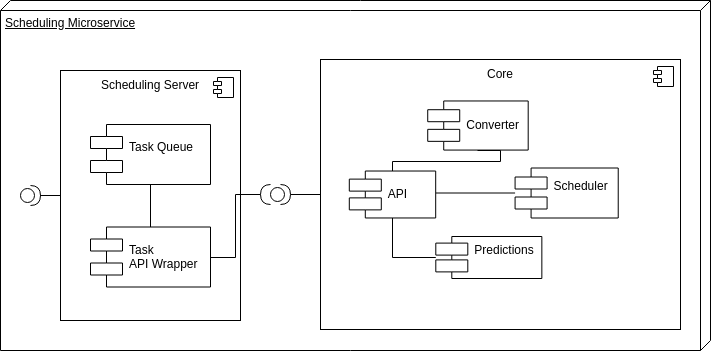
\includegraphics[width=\textwidth]{i_scheduler.png} 
    \centering
    \caption{Microservice architecture with scheduling core}
    \label{fig:scheduling-core-arch}
\end{figure}

Core component, 
which is responsible for scheduling and load balancing,
is composed of API, converter, predictions and scheduler module.
\begin{itemize}
    \item \textit{API module} implements common core interface \inlinecode{OlbCoreApi} 
    and is responsible for scheduling requests handling.
    Actual implementation of API interface is class \inlinecode{OlbCoreApiImpl}.
    \item \textit{Converter module} is used to convert received input data into inner scheduler data representation 
    and then back to common data transfer objects. 
    This converter is implemented as a class \inlinecode{InputToDomainConverter}.
    \item \textit{Scheduler module} contains constraints, evaluator and scheduling system based on OptaPlanner solution
    (described in section \ref{sec:load-balancing-optaplanner}).
    Scheduler module consist of multiple packages, 
    \inlinecode{constraints} - containing all constrains for scheduling algorithm,
    \inlinecode{domain} with defined scheduling domain for OptaPlanner,
    \inlinecode{evaluation} which includes evaluator calculating planning score
    and \inlinecode{solver} package with factory initializing OptaPlanner scheduling core.
\end{itemize}

Scheduling server provides HTTP API access to the core
and serves as microservice base.
Server module is based on Ktor framework (described in section \ref{subsec:framework})
that runs under the hood and provides HTTP functionality.

In the current implementation,
server API accepts binary serialized data transfer objects
instead of common JSON or XML.
This is because of number of interfaces and loosely coupled data objects,
that are being used in the application.
Migration to JSON technology is addressed in future work in section \ref{sec:future-work}.

\subsubsection{Simulations architecture}\label{subsec:simulations-architecture}
Simulations module (project module \inlinecode{simulations}) is designed as another microservice to simulate future load balancing system's behavior.
Following figure \ref{fig:simulations-arch} shows architecture of the module.  

\begin{figure}[ht]
    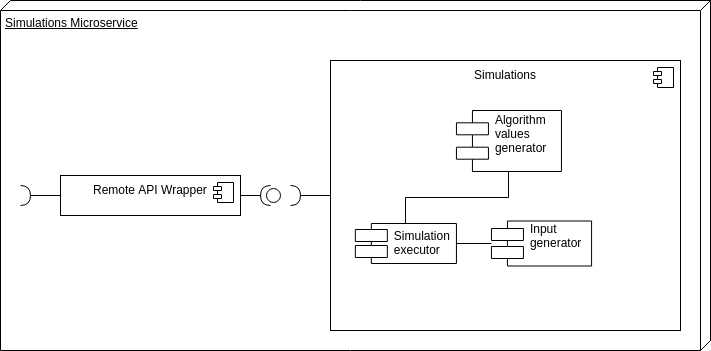
\includegraphics[width=\textwidth]{i_simulations.png}
    \centering
    \caption{Simulations module scheme}
    \label{fig:simulations-arch}
\end{figure}

Input data are generated by input generator module,
which can be found for example in \inlinecode{DomainBuilder} class.
Algorithm values are parsed from file in class \inlinecode{DataParser} 
and corresponding model is created on top of them in \inlinecode{JobWithHistoryFactory}.

Remote API wrapper is used to create connection between remote microservice, with scheduling API, and simulation.
For the simulation module,
the connection seems to be synchronous.
This is because there is a blocking queue used to store and answer the calls between these two microservices.
Thanks to this solution,
simulations can be run in microservices mode as well as locally without any additional effort needed.
Remote scheduling solution is implemented in project module \inlinecode{remote-scheduler}.
Local simulations can be found for example in \inlinecode{OnePlanningRoundMain} or \inlinecode{ExecutionConfiguration} classes.

\section{Related and used technologies}\label{sec:related-technologies}
General information about used technologies.

\subsection{Java platform}\label{subsec:tech-java}
general info about java programming language and java paltform

\subsection{Docker}\label{subsec:tech-docker}
Docker is a technology that performs operating-system-level virtualization,
meaning that it uses hosts operating system kernel
general info about docker 

\section{Development stack}\label{sec:development-stack}
The development stack is based on the Java platform, 
targeting primarily JVM 11\footnote{Java Virtual Machine - runtime environment for Java byte code}
but including backwards compatibility with JVM 8.
However, 
the traditional Java platform programming language Java was not used.

\subsection{Programming Language}\label{subsec:programming-language}
The OLB\footnote{Optimization Load Balancer, name of the application} is not bound to the single technology, 
which could limit the development stack and for that reason,
we had a free choice while choosing the programming language used for the OLB implementation.

OLB is programmed in the programming language \textbf{Kotlin}.
This cross-platform, statically typed, the general-purpose programming language is developed by JetBrains\cite{kotlinReference}.
Kotlin is 100\% interoperable with Java because it uses JVM as its runtime and it is compiled to the Java Bytecode.
Apart from the Java Bytecode, it can also be compiled to JavaScript or native code.\cite{kotlinReference}
The main advantage of Kotlin is its aggressive and robust type inference,
meaning that for the most of the time,
it is not necessary to specify used data type since Kotlin compiler can infer it from the context.\cite{kotlinReference}
It results in concise language syntax and therefore to the faster development in general.

Another great advantage is Kotlin's \textit{null safety}. 
Kotlin compiler distinguishes between non-nullable types and nullable types 
and enforces \textit{null checks}\footnote{Check whether the object being used has not null value} when the object has a nullable data type.
This feature effectively leads to fewer problems in the code
and drastically reduces \textit{Null Pointer Exceptions}\footnote{Exception raised when code access reference that has null value}
during the runtime.

\subsection{Build environment}
The application uses Gradle as its build automation system.
It was chosen mainly because its incrementally build system,
that works by tracking input and output of tasks, 
including files changes tracking, and only running tasks, that are necessary
and thus reducing the required time to build the project. 
Also, it processes only these files that were changed between tasks execution. 
Another reason we choose Gradle was that it is preferred build system for Kotlin.

The preferred approach to assemble the application is to use Docker
and build it as the Docker image, 
which can be then run inside the Docker container.

\subsubsection{Docker build environment}
To keep the build clean and reusable on almost every operating system and 
machine setup we decided to use 
\textbf{multistage Docker build}\footnote{Docker is a technology that performs operating-system-level virtualization,
meaning that it uses hosts operating system kernel}
which uses different base docker images for the build and the run phase.
Since OLB targets the JVM 11 environment and uses Gradle as its build system,
\textit{gradle:5.4.0-jdk11-slim} is used as base image for build stage.
This image contains all necessary Gradle build tools while having a smaller size than the common Gradle Docker image.
Even smaller (in terms of size) are \textit{alpine} based docker images. 
Alpine is the smallest possible Linux core, 
which is widely used in the full range of Docker base images.
Alpine is focused on the smallest possible size of the image, 
while having all the necessary tools built in.
Unfortunately, there were (at the time of development) no official JVM 11 alpine images
since there is no official stable OpenJDK\footnote{Open-source implementation of the Java Platform, Standard Edition} 
11 build for Alpine Linux.

\subsection{Runtime environment}
The preferred runtime environment is a Docker system, 
where the application image runs inside the created docker container.

\subsubsection{Docker runtime environment}\label{subsubsec:docker-runtime-env}
The build application files are copied from the Docker build stage to the Docker runtime stage.
As the runtime base image in the multistage build was used \textit{openjdk:11-jre-slim} image,
because it is an official OpenJDK 11 Docker image and therefore it is declared as stable.

Because there was used \textit{gradle application plugin} while building the application, 
startup scripts were generated by the Gradle.
These scripts are then used to start the application itself inside the Docker container.

When starting the whole application, 
multiple services must be started up.
Therefore, because of the containerized environment,
where containers can not access each other,
multiple containers must be started, and the virtual network connecting them must be created.
This process can be automated using Docker Compose.

\subsubsection{Docker Compose}
Docker Compose\cite{dockerComposeReference} is an application for defining, running and managing multi-container Docker applications.
It automatically creates Docker networks as well as Docker volumes.
With writing down the definition of multiple Docker applications to the one Docker Compose configuration file,
it is possible to create robust microservices architecture, 
which can be built or started using a single command.

Thanks to the created Docker networks,
containers can communicate with each other using Docker Compose service names,
therefore they do not need to know specific IP address they have.

Docker Compose is used in the implementation of OLB since it is designed with microservices architecture in mind.
There are two services - Scheduling server and Scheduling client.
Scheduling server provides the ability to schedule process execution on the various computers
and contains all core algorithms.
Scheduling client is an example application which uses the ability of scheduling server. 
There are implemented various simulations,
which are being executed by scheduling client.  

\subsection{Framework}\label{subsec:framework}
Because of the overall microservices architecture of the project,
a web framework was needed.
There are many Java-based web frameworks 
that could be used. 
We would like to present two of them - \textit{Spring Boot}, 
which is a traditional and widely used web framework for all kind of Java web applications
and \textit{Ktor} - relatively new, 
lightweight Kotlin framework build upon the Kotlin Coroutines\footnote{Way of asynchronous or non-blocking programming
that generalize subroutines for non-preemptive multitasking with using suspended/resumed task execution}.


\subsubsection{Spring Boot}
Spring Boot\cite{springBootReference} is an open source Java Spring-powered web framework.
It takes an opinionated view of the Spring platform,
meaning that Spring Boot automatically configure Spring and 3rd party libraries whenever possible,
and therefore enables usage of it to broader audience.
It is highly dependent on the starter templates feature which provides pre-configured templates for various types of web applications.
This, for example, allows the user to start with already working web server
and thus simplify the start of the application development\cite{springBootGithubReference}.
Spring Boot contains comprehensive infrastructure support for developing enterprise monolith web applications as well as micro services\cite{springBootGithubReference}.

\subsubsection{Ktor}\label{subsubsec:ktor}
Ktor \cite{ktorWebPage} is an open source web framework for building asynchronous servers 
and clients in connected systems such as web applications and HTTP services.
It designed for quickly building web applications with minimal effort 
and it doesn't impose a lot of technical constraints such as logging, persistent, serializing, dependency injection etc.\cite{ktorApiReference}
It is developed by the same company as Kotlin is, JetBrains.


\bigskip
The final decision was to use \textbf{Ktor} as the web framework,
mainly because of its very light implementation and native Kotlin support.
Also, for such a project, 
the features of Spring would not be fully utilized
and therefore, the complexity of Spring could potentially slow down the entire application.

Because Ktor by default does not contain any dependency an injection framework, 
We decided to use lightweight DI\footnote{Dependency Injection} framework \textit{Koin}\cite{koinGithub}.
This framework is written in Kotlin and have its own DSL\footnote{Domain Specific Language} for the dependency specification,
which is very handy for the medium-sized project.

\subsubsection{Route discovery library}
The default way, how to create a HTTP endpoint (Ktor calls them \textit{routes}),
which can handle HTTP requests is registering it within the \inlinecode{Application} context.
The \inlinecode{Application} context is accessible by its instance that is given to the user when the Ktor is being started.
This means that no \textit{route} can be registered without using an instance of \inlinecode{Application}.

During the development of the application and using Ktor framework, 
we decided that the proprietary way of registering routes was not something we would like to be using,
mainly because it did not allow to have pure class serving only as a route without having to inject the \textit{Application} instance.
Also, 
since the routes must be registered during the application startup,
using the new class for each route would mean to create an instance of the class and executing the method to register the routes manually.
Another reason we did not like the Ktor default approach was 
that we prefer to inject class dependencies using the construct injection instead of using the setters injection.
\begin{itemize}
    \item Constructor dependency injection - using the constructor of the class to set all instances of the objects, that class uses.
          The main advantage is that the instance of the class is always in a valid state because it has all dependencies resolved during the instance creation.
    \item Setter dependency injection - the dependent objects are provided by the setter methods.
          This gives the freedom to manipulate the state of the dependency references at any time.
          However, it is possible to use the instance without setting the dependencies which could lead to the undefined behavior or the \textit{Null Pointer Exceptions}
\end{itemize}

To solve this \inlinecode{Application} instance dependency and to enable constructor dependency injection approach,
we decided to implement a simple library which would solve this issue for us.
We came up with a different way how to register various types of application's routes using the annotations, 
reflection and dependency injection strategy.

\medskip \noindent
Preconditions for successful usage of the library are the following:
\begin{itemize}
    \item \textit{Koin}\cite{koinGithub} - dependency injection framework which is used for resolving dependencies needed in the routes
    \item \textit{Reflection library}\cite{reflectionsGithub} - library used for runtime lookup for classes with specific annotation
    \item Using the \inlinecode{@Route} annotation on the class that is meant to be route,
    the class has to also inherit from \inlinecode{RouteBase}
    \item Registering all necessary routes dependencies in \textit{Koin} modules during the application startup
    \item Provide base package name where routes are placed.
\end{itemize}

\medskip \noindent
Following algorithm is used to find and register all routes used in the project.

\begin{algorithm}[H]
    \SetAlgoLined
    \Input{Package name, where all routes are stored}
    \textbf{routes} $\leftarrow$ find all classes annotated as \inlinedata{@Route} in provided package name\;
    \For{\textbf{route} in \textbf{routes}}{
        \textbf{dependencies} $\leftarrow$ obtain dependencies needed for creating instance of \textbf{route}\;
        \textbf{routeInstance} $\leftarrow$ create instance of \textbf{route} using \textbf{dependencies}\;
        register \textbf{routeInstance} in instance of \inlinedata{Application} \;
    }
    \Output{All routes are registered and ready to use}
\end{algorithm} 
\medskip \noindent
The implementation of the simple route is then following:

\medskip
\begin{samepage}
\begin{lstlisting}[language=Kotlin]
@Route
class HelloRoute(sr: Service) : RouteBase("hello") {
    init {
        route {
            get {
                call.respond(sr.sayHello())
            }
        }
    }
}
\end{lstlisting}
\end{samepage}

\medskip \noindent
The route is automatically instantiated and registered by the Routes discovery library.
The programmer does not need to handle it by himself.

For the library startup, we designed a builder class using fluent builder pattern \inlinecode{ApplicationDependencyBuilder}.
Usage of this class can be found in the \inlinecode{ServerStarter.kt}.

\section{Algorithm value prediction}\label{sec:algorithm-value-prediction}

To have the most informed decisions while creating load balancing decisions,
algorithm creating these decisions should be able to estimate impact of assigned resources to the job-value development.
Unfortunately, 
it is not possible to exactly predict the value function,
because for instance optimization algorithms based on heuristics and metaheuristics are stochastic 
and therefore there is no guarantee that they will eventually find a better solution
or how fast they will be able to do that.
That said, 
the only thing that is guaranteed is that the job value function over time period is monotonically non-increasing.

However,
since it is not necessary to have exact prediction values,
we can roughly approximate the job value function as the hyperbola function.
Using this approximation means,
that value prediction algorithm is trying to fit time series data into hyperbola.\todo{check this expression, it does not seems right}

Moreover, 
it is not possible to use the time as $x$ axis,
because it would not be possible to extract information about 
how adding more available performance will modify the predicted job value function.
For that reason,
it is better to use the number of iterations, that optimization algorithm performed,
instead of time unit.

\subsection{Hyperbola time series fitting}
The generic equation for expressing hyperbola function on two dimensional graph is following.
\begin{equation}
    a + \dfrac{b}{x+c} = y
\end{equation}
Where $a,b,c$ are parameters and $x,y$ are axis values.
For usage in computer algorithm,
it is better to transform the equation into the form, 
where there is no division.
Apart from the better performance in favor of multiplication\cite{LeFevre1999},
it is possible that the state when $x = -c$ occurs.
If there is the division,
the resulting value will be infinity,
which breaks next algorithm iterations.

Instead,
it is better to use following form, 
where there is no division and $0$ as a result is not a problem for the following algorithm iterations.
\begin{equation}\label{eq:final-hyperbola-fc}
    ax + ac + b - yc = yx
\end{equation}

Since the algorithm value prediction should be computed as fast as possible
and it is not necessary to have the precise value,
I decided to use mathematics optimization approach transforming the problem into non-linear least squares problem.

Non-linear least squares problems are often solved by the iteration algorithms 
such as Gauss-Newton algorithm\cite{gratton2007approximate} and Levenberg–Marquardt algorithm\cite{marquardt1963algorithm}.
The second mentioned non-linear algorithm is more robust than the Gauss-Newton, 
because of the Marquardt parameter\cite{marquardt1963algorithm},
which means that in many cases it finds a solution even if it starts very far off the final minimum.

Using Levenberg–Marquardt algorithm means, 
that it is necessary to know the derivation of the function, 
algorithm is trying to fit in.
Derivation of the used function \ref{eq:final-hyperbola-fc} is then following.
\begin{equation}\label{eq:final-hyperbola-fd}
    f'(x) = (c+x, 1, a-y)
\end{equation}

As the target values, are used $x \cdot y$.
As the parameters, that Levenberg–Marquardt algorithm is trying to fit in are used $a,b,c$.

\section{Load balancing decisions}\label{sec:load-balancing-decisions}

Used library - https://www.optaplanner.org/


\section{OLB Algorithm}\label{sec:olb-algorithm}
how this shit works

    \bibliographystyle{amsalpha}
    \bibliography{report}
\end{document}